\section{Regression}
Linear Regression is \textbf{Supervised Learning} and subclass \textbf{Regression}.
\subsection{What is a model?}
In ML, we use the term \textbf{model} for any mathematical function that explains the data:\\
$y_i = f(x_i)$\\
$y_i = f(x_i) + \epsilon_i$\\
where $\epsilon_i$ is unexplained noise. It is often assumed that $\epsilon_i$ follows a normal distribution.\\
Instead of approximating $y_i$, we calculate an \textbf{estimate} $\hat{y_i}$ (y hat) of the usually unknown $y_i$: \\
\begin{center}
    $\hat{y_i} = f(x)$
\end{center}

\subsection{Linear Regression}
In ML, linear regression falls into the category of supervised learning.
\textbf{Two categories:}\\
\textbf{Interpretation:} We want to understand if some input has an effect on the output. Example: Is there a
relationship between smoking cigaretts and the risk of lung cancer?\\
\textbf{Prediction:} Given some sensor data like oil pressure, temperature etc. a model could predict (and thereby
hopefully prevent) an engine failure.     <<

\begin{itemize}
    \item Only considers a linear relationship between input and output
    \item In the simplest case, $x$ and $y$ are scalars and the linear model therefore has only two free parameters
    \item The goal is to identify $a$ (slope) and $b$ (intercept) for which the linear model best explains the data
\end{itemize}
\textbf{Examples:}\\
Linear: $\hat{y_i} = ax_i + b$\\
Squared: $\hat{y_i} = w_2 * x_i^2 + w_1 * x_i + w_0$\\
Cubic: $\hat{y_i} = w_3 * x_i^3 + w_2 * x_i^2 + w_1 * x_i + w_0$\\


\subsubsection{Mean Squared Error (MSE)}
\begin{itemize}
    \item Loss we want to minimize
    \item Usually divided by 2
\end{itemize}
    $$e_i = y_i - \hat{y_i}$$
    The difference $e_i$, called \textbf{residual}.\\
    (Value between linear function and datapoint)
    $$MSE = \frac{1}{2N} * \displaystyle\sum_{i = 1}^{N} e_i^2$$
    $$MSE = \frac{1}{2N} * \displaystyle\sum_{i = 1}^{N} (y_i - \hat{y_i})^2$$\\
    Einsetzten:
    $$\hat{y_i} = ax_i + b$$
    $$E = \frac{1}{2N} * \large\displaystyle\sum_{i = 1}^{N}({y_i} - (a*x_i + b))^2$$

\subsection{Correlation and Causality}
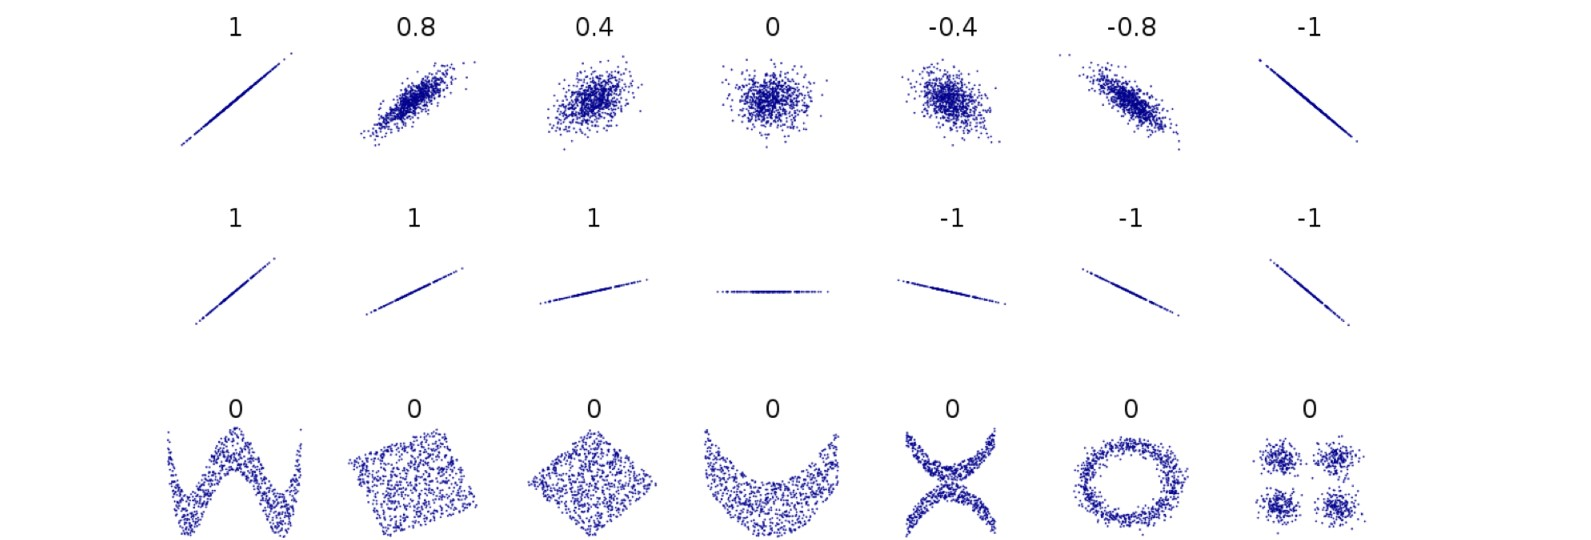
\includegraphics[width=\linewidth]{pearson.jpg}
\begin{itemize}
    \item Correlation is not causality
    \item Correlation refers to the degree to which a pair of variables are linearly related
    \item Linear regression is a tool to detect correlations between two or more variables
    \item Correlation can be quantified using the Pearson correlation coefficient
    \item Even if the correlation coefficient is 0, the data can still be highly structured
\end{itemize}

\subsection{Complex linear models}
We can have linear models that depend on more than one input variable.
In this case, x is a vector with p features (=dimensions):
\begin{center}
    $y_i = \beta_0 + \beta_1 x_{i1} + \beta_2 x_{i2} + \beta_3 x_{i3} + \dots + \beta_p x_{ip}$
\end{center}
For many data ($x_i,y_i$) we can express the linear model in matrix notation:
\begin{center}
    $X\beta = y$
\end{center}